\documentclass[honours,12pt,twoside]{unswthesis}

\usepackage{afterpage}
\usepackage{amsfonts}
\usepackage{amsmath}
\usepackage{amssymb}
\usepackage{amsthm}
\usepackage[english]{babel}
\usepackage{graphicx}
\usepackage{natbib}
\usepackage[utf8]{inputenc}
\usepackage{latexsym}
\usepackage{url}
\usepackage{todonotes}
\usepackage{tikz}
\usepackage{pdfpages}
\usetikzlibrary{arrows}
\usepackage{float}

\usepackage{booktabs}
\renewcommand{\arraystretch}{1.2}


%%%%%%%%%%%%%%%%%%%%%%%%%%%%%%%%%%%%%%%%%%%%%%%%%%%%%%%%%%%%%%%%%
%
%  The following are some simple LaTeX macros to give some
%  commonly used letters in funny fonts. You may need more or less of
%  these
%
\newcommand{\R}{\mathbb{R}}
\newcommand{\Q}{\mathbb{Q}}
\newcommand{\C}{\mathbb{C}}
\newcommand{\N}{\mathbb{N}}
\newcommand{\F}{\mathbb{F}}
\newcommand{\PP}{\mathbb{P}}
\newcommand{\T}{\mathbb{T}}
\newcommand{\Z}{\mathbb{Z}}
\newcommand{\B}{\mathfrak{B}}
\newcommand{\BB}{\mathcal{B}}
\newcommand{\M}{\mathfrak{M}}
\newcommand{\X}{\mathfrak{X}}
\newcommand{\Y}{\mathfrak{Y}}
\newcommand{\CC}{\mathcal{C}}
\newcommand{\E}{\mathbb{E}}
\newcommand{\cP}{\mathcal{P}}
\newcommand{\cS}{\mathcal{S}}
\newcommand{\A}{\mathcal{A}}
\newcommand{\ZZ}{\mathcal{Z}}

%%%%%%%%%%%%%%%%%%%%%%%%%%%%%%%%%%%%%%%%%%%%%%%%%%%%%%%%%%%%%%%%%%%%%
%
% The following are much more esoteric commands that I have left in
% so that this file still processes. Use or delete as you see fit
%
\newcommand{\bv}[1]{\mbox{BV($#1$)}}
\newcommand{\comb}[2]{\left(\!\!\!\begin{array}{c}#1\\#2\end{array}\!\!\!\right)
}
\newcommand{\Lat}{{\rm Lat}}
\newcommand{\var}{\mathop{\rm var}}
\newcommand{\Pt}{{\mathcal P}}
\def\tr(#1){{\rm trace}(#1)}
\def\Exp(#1){{\mathbb E}(#1)}
\def\Exps(#1){{\mathbb E}\sparen(#1)}
\newcommand{\floor}[1]{\left\lfloor #1 \right\rfloor}
\newcommand{\ceil}[1]{\left\lceil #1 \right\rceil}
\newcommand{\hatt}[1]{\widehat #1}
\newcommand{\modeq}[3]{#1 \equiv #2 \,(\text{mod}\, #3)}
\newcommand{\rmod}{\,\mathrm{mod}\,}
\newcommand{\p}{\hphantom{+}}
\newcommand{\vect}[1]{\mbox{\boldmath $ #1 $}}
\newcommand{\reff}[2]{\ref{#1}.\ref{#2}}
\newcommand{\psum}[2]{\sum_{#1}^{#2}\!\!\!'\,\,}
\newcommand{\bin}[2]{\left( \begin{array}{@{}c@{}}
				#1 \\ #2
			\end{array}\right)	}
%
%  Macros - some of these are in plain TeX (gasp!)
%
\newcommand{\be}{($\beta$)}
\newcommand{\eqp}{\mathrel{{=}_p}}
\newcommand{\ltp}{\mathrel{{\prec}_p}}
\newcommand{\lep}{\mathrel{{\preceq}_p}}
\def\brack#1{\left \{ #1 \right \}}
\def\bul{$\bullet$\ }
\def\cl{{\rm cl}}
\let\del=\partial
\def\enditem{\par\smallskip\noindent}
\def\implies{\Rightarrow}
\def\inpr#1,#2{\t \hbox{\langle #1 , #2 \rangle} \t}
\def\ip<#1,#2>{\langle #1,#2 \rangle}
\def\lp{\ell^p}
\def\maxb#1{\max \brack{#1}}
\def\minb#1{\min \brack{#1}}
\def\mod#1{\left \vert #1 \right \vert}
\def\norm#1{\left \Vert #1 \right \Vert}
\def\paren(#1){\left( #1 \right)}
\def\qed{\hfill \hbox{$\Box$} \smallskip}
\def\sbrack#1{\Bigl \{ #1 \Bigr \} }
\def\ssbrack#1{ \{ #1 \} }
\def\smod#1{\Bigl \vert #1 \Bigr \vert}
\def\smmod#1{\bigl \vert #1 \bigr \vert}
\def\ssmod#1{\vert #1 \vert}
\def\sspmod#1{\vert\, #1 \, \vert}
\def\snorm#1{\Bigl \Vert #1 \Bigr \Vert}
\def\ssnorm#1{\Vert #1 \Vert}
\def\sparen(#1){\Bigl ( #1 \Bigr )}

\newcommand\blankpage{%
    \null
    \thispagestyle{empty}%
    \addtocounter{page}{-1}%
    \newpage}
    
%%%%%%%%%%%%%%%%%%%%%%%%%%%%%%%%%%%%%%%%%%%%%%%%%%%%%%%%%%%%%%
%
% These environments allow you to get nice numbered headings
%  for your Theorems, Definitions etc.  
%
%  Environments
%
%%%%%%%%%%%%%%%%%%%%%%%%%%%%%%%

\newtheorem{theorem}{Theorem}[section]
\newtheorem{lemma}[theorem]{Lemma}
\newtheorem{proposition}[theorem]{Proposition}
\newtheorem{corollary}[theorem]{Corollary}
\newtheorem{conjecture}[theorem]{Conjecture}
\newtheorem{definition}[theorem]{Definition}
\newtheorem{example}{Example}
\newtheorem{remark}[theorem]{Remark}
\newtheorem{question}[theorem]{Question}
\newtheorem{notation}[theorem]{Notation}
\numberwithin{equation}{section}

\begin{document}

\chapter{Results}\label{results}

\section{Final model structure}

The final simplified model has a similar structure to that of Ghafoorian et. al's candidate detection model \cite{GhafoorianM.2017Dml3}. The model structure is shown in Figure \ref{results-model-fig}. The input data contains two axial images: soft-tissue extracted T1 and FLAIR, each of resolution 51$\times$51 pixels around the same point. The model classifies the central pixel as either a positive or negative reading, formatted as a 2-dimensional vector. A response of $(1,0)^\intercal$ indicates a positive (lacune) and $(0,1)^\intercal$ a negative (non-lacune).

% Simplified model structure
\begin{figure}[ht]
	\centering
	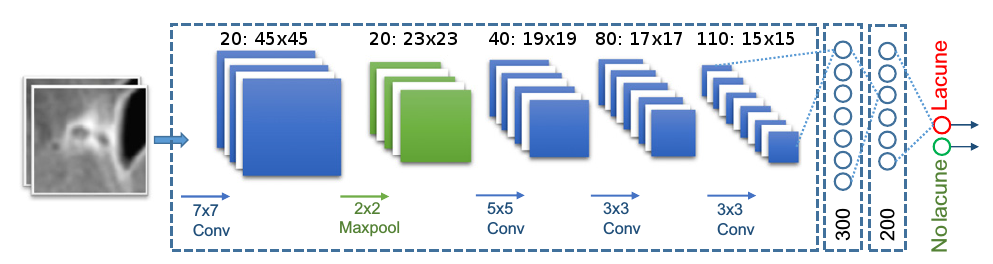
\includegraphics[width=\textwidth]{Images/7_simplified_model.png}
	\caption{Simplified model structure.}
	\small Image adapted from \cite{GhafoorianM.2017Dml3}
	\label{results-model-fig}
\end{figure}

The model consists of four convolutional layers of size 20, 40, 80 and 110, with filter sizes 7$\times$7, 5$\times$5, 3$\times$3 and 3$\times$3 respectively. A single max pooling layer is placed after the first convolutional layer, with size 2$\times$2 and stride 2. The convolutional layers are followed by three fully connected layers of size 300, 200 and 2. The final layer has softmax activation to output a probability distribution. All other layers have ReLU activation in order to avoid the vanishing gradient problem (see Section \ref{nnet-vanishinggradprob}).

All neurons undergo batch normalisation and are initialised using the He method \cite{HeK2016Drlf}. A dropout rate of 0.3 was applied to the fully connected layers.

Training was conducted using stoachastic gradient descent with Adam optimiser and a batch size of 128. A decaying learning rate was set from $5\times10^{-4}$ to $1\times10^{-6}$ by the 40th epoch. Cross-entropy loss was used with L2-regularisation. The penalty rate was set to $1\times10^{-4}$. 

An early stopping mechanism was implemented such that the model is tested against the validation set at the end of each epoch. If the validation accuracy improves, the model is saved. Once 40 epochs have run, the final saved model will have the highest validation accuracy.

Two models were trained using different positive-negative response ratios. The first model was developed using the positive-negative response ratio described by Ghafoorian et. al \cite{GhafoorianM.2017Dml3}: one third positive and two thirds negative. There are only 3846 positive samples in the MAS dataset, allowing for a random selection of 7692 negative samples. The total sample size is 11538. These samples are split into three datasets: training, validation and testing. Splitting the data into these groups with a ratio of 50:25:25 yields sample sizes 5769, 2884 and 2885 respectively.

The second model used the entire developed set of positive and negative lacune samples. This consisted of 3846 positive and 40008 negative samples to give a total sample size of 43854. Positives encompassed 8.77\% of data samples. Similarly to the first dataset, the data was split into training, validation and testing sets using a ratio of 50:25:25. This yielded sample sizes 21927, 10963 and 10964 respectively. All datasets were saved as R data files (\texttt{.Rda}).


\section{Training environment}

Model code was developed in R (v3.5.0) using RStudio (v1.1.453). The neural network was built and trained using Tensorflow (v1.10.0) through the R interface \texttt{tensorflow} (v1.8). The model was trained on a Linux machine running Ubuntu (release 16.04). 

\section{Results}

The first model generated had the same positive-negative sample ratio as outlined by Ghafoorian et. al \cite{GhafoorianM.2017Dml3}. The data consisted of one third positives and two thirds negatives. The resulting samples were split into three datasets: training, validation and testing in the ratio of 50:25:25.

Training accuracy was calculated every 5 batches, where each batch contains 128 samples. Validation accuracy was calculated at the end of each epoch. The model trained for 40 epochs in 23 minutes. Training accuracy, shown in Figure \ref{results-train-acc-fig}, increased rapidly in the first 100 batches. Training accuracy first reach 100\% by batch 
% Training accuracy
\begin{figure}[ht]
	\centering
	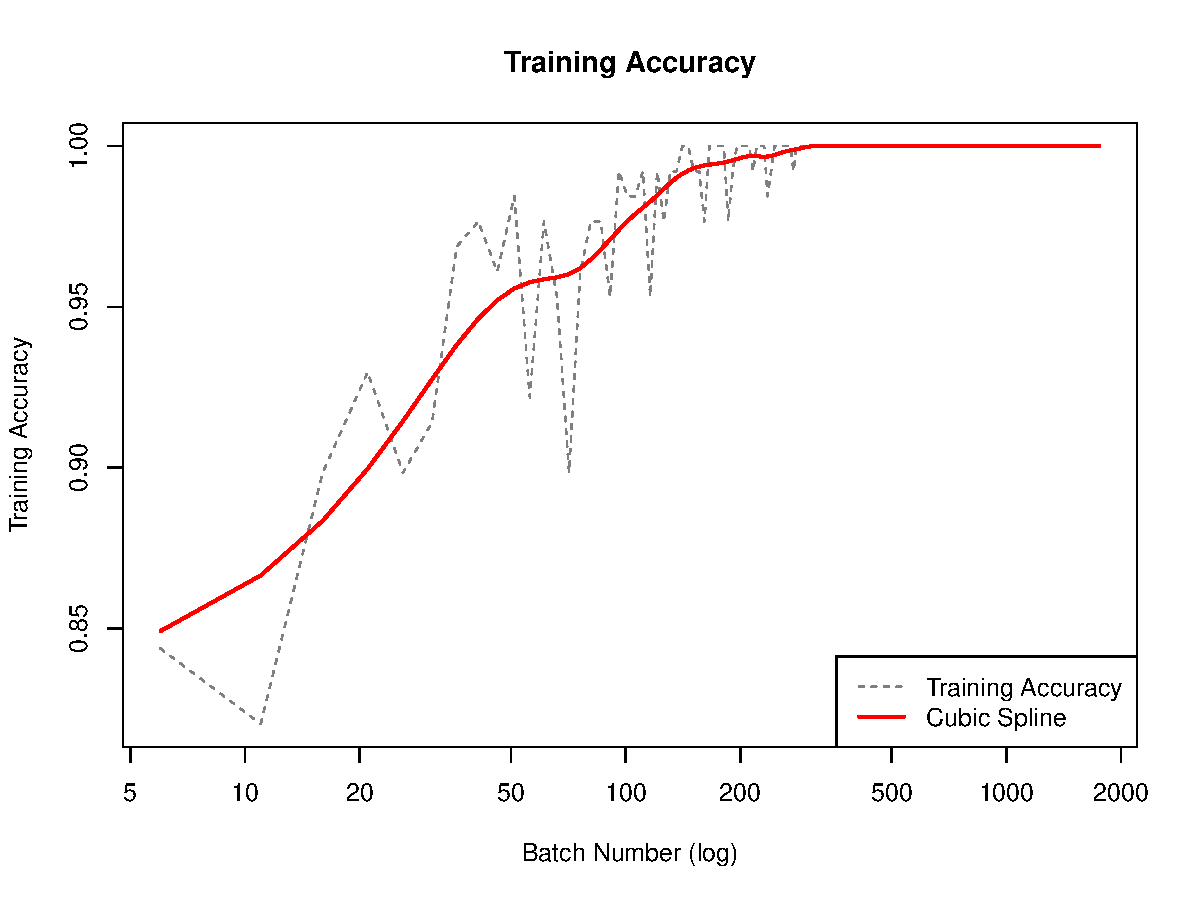
\includegraphics[width=\textwidth]{Images/7_train_acc4.pdf}
	\caption{Training data accuracy logged every 5 batches}
	\label{results-train-acc-fig}
\end{figure}

%\section{Reference Model Results}
%
%Results from running Ghafoorian's model. Training time, and final sensitivity and average false-positives per slice.
%
%\subsection*{Attempt1}
%
%training/testing in ratio 70:30. Here, only 7\% of data consists of positives. 41819 samples in total. Validation occurs on first 500 of the testing set. Training time: 02:04:48.
%Training accuracy achieved 100\% before batch 100x5. Validation accuracy peaked at epoch 8, with an accuracy of 100\%. Though should be noted that the size of this validation set consists of only 500 samples. Testing the whole testing set (15544 samples) achieves an accuracy of 0.9938.
%
%\subsection*{Attempt2}
%
%training/validation/testing in ratio 50:25:25. 1/3 of data was positives. 11539 samples in total. Training time: 00:23:11.
%Training accuracy achieved 100\% before batch 50x5. Validation accuracy peaked at epoch 21, which achieved an accuracy of 0.984055. Applying this best validation model to testing data achieved an accuracy of 0.9833622. Lower accuracy could be the result of fewer data points for training - caused by having only a limited number of positives in the original dataset compared to the abundant negatives.
%
%\subsection*{Attempt3}
%
%Use original 7\% ratio. 41819 samples, with training/validation/testing in ratio 50:25:25. Have to be careful not to introduce too many negatives as this could impact what the model attempts to predict. E.g. if there are only 1\% positives, then an accuracy of 99\% could be achieved just by labelling all the samples as negative. Training time: 01:58:23.
%Training accuracy achieved 100\% before batch 100x5. Validation accuracy peaked at epoch 18, with an accuracy of 0.9979159, with the set containing 12955 samples. The testing set achieved an accuracy of 0.9972.
%
%\subsection*{Fixed Samples}
%
%Samples were changed. Previously, negative samples were chosen such that they were not lacunes, and also did not have a central pixel value of 0. However, some regions within the brain matter do have a central value of 0, and these can be some of the hardest points to distinguish.
%
%Negative sampling was changed to random points that were not lacunes, and the entire 9x9 central square is not 0 (to remove samples from outside the brain matter). 
%
%\subsection*{Attempt4}
%
%training/validation/testing in ratio 50:25:25. 1/3 of data was positives. 11538 samples in total. Training time: 00:22:51.
%Training accuracy achieved 100\% at batch 28x5. Consistent 100\% by batch 50x5. Validation accuracy peaked at epochs 31 and 34, achieving an accuracy of 0.9899445. Applying this best validation accuracy model to the test set achieved an accuracy of 0.9885615.
%
%Testing set was only 2885 samples. The number of true/false positives and negatives were:
%TP: 972
%TN: 1879
%FP: 30
%FN: 4
%
%Sensitivity is 972/(972+4) = 99.6\% and specificity is 1879/(1879+30) = 98.4\%.
%
%
%
%\subsection*{Attempt5}
%
%training/validation/testing with 8.77\% positives. 43854 samples in total. Training time: 01:13:17. Training accuracy achieved 100\% at batch 41x5. Consistently 100\% at batch 150x5. Validation accuracy peaked at epoch 22, which achieved an accuracy of 0.9983581. Applying this best validation accuracy model to the test set achieved an accuracy of 0.9968989.
%Testing set comprised of 10964 samples. Of these, the number of true/false positives and negatives were calculated:
%
%TP: 955
%TN: 9969
%FP: 33
%FN: 7
%
%Sensitivity is 955/(955+7) = 99.3\%, and specificity is 9969/(9969+33) = 99.7\%.

%%%%%%%%%%%%%%%%%%%%%%%%%%%%%%%%%%%%%%%%%%%%%%%%%%%%%%%%%%%%%%%%%%%%%%%%%%

\clearpage

\addcontentsline{toc}{chapter}{References}

\bibliographystyle{apalike}
\bibliography{bibliography.bib}

%\bibliographystyle{apacite}
%\bibliography{mybib.bib}

